\section{LED}
\subsection{PWM-Signale}\label{Appendix:Timer_PWM}

Das PWM-Signal für die LEDs wird mit einer Frequenz von 10 kHz initialisiert. Um dies zu erreichen, wird Formel \ref{equ:Timer_Max_1} umgestellt nach \ref{equ:Timer_Max_2}. Der Prescaler ist N = 1. Das Ergebnis wird im Register OCRnA gespeichert, wodurch der Timer $1/10kHz = 100\mu s$ benötigt, bis ein Timer\_nA Compare-Interrupt ausgelöst wird. \cite[S.148]{atmel_atmel_2014}

\begin{equation}
f_{OC_{nA}PWM} = \frac{f_{clk_{I/O}}}{N \cdot (1+OCR_{nA})}
\label{equ:Timer_Max_1}
\end{equation}

umgestellt nach OCR\_nA:

\begin{equation}
OCR_{nA} = \frac{f_{clk_{I/O}}}{N \cdot f_{OC_{nA}PWM}} - 1 = \frac{16MHz}{1 \cdot 10kHz} - 1 = 1599
\label{equ:Timer_Max_2}
\end{equation}

Damit das Hochzählen des Counters nach erreichen von OCRnA wieder bei null beginnt, wird der Timer im CTC-Mode betrieben. Das Register OCRnA stellt so den maximalen Wert des Counters dar. Dies ist in Abbildung \ref {fig:Timer_CTC_Mode} und \ref{fig:Timer_CTC_Timing_Diagram} zu sehen.

\begin{figure}[h!]
	\centering
	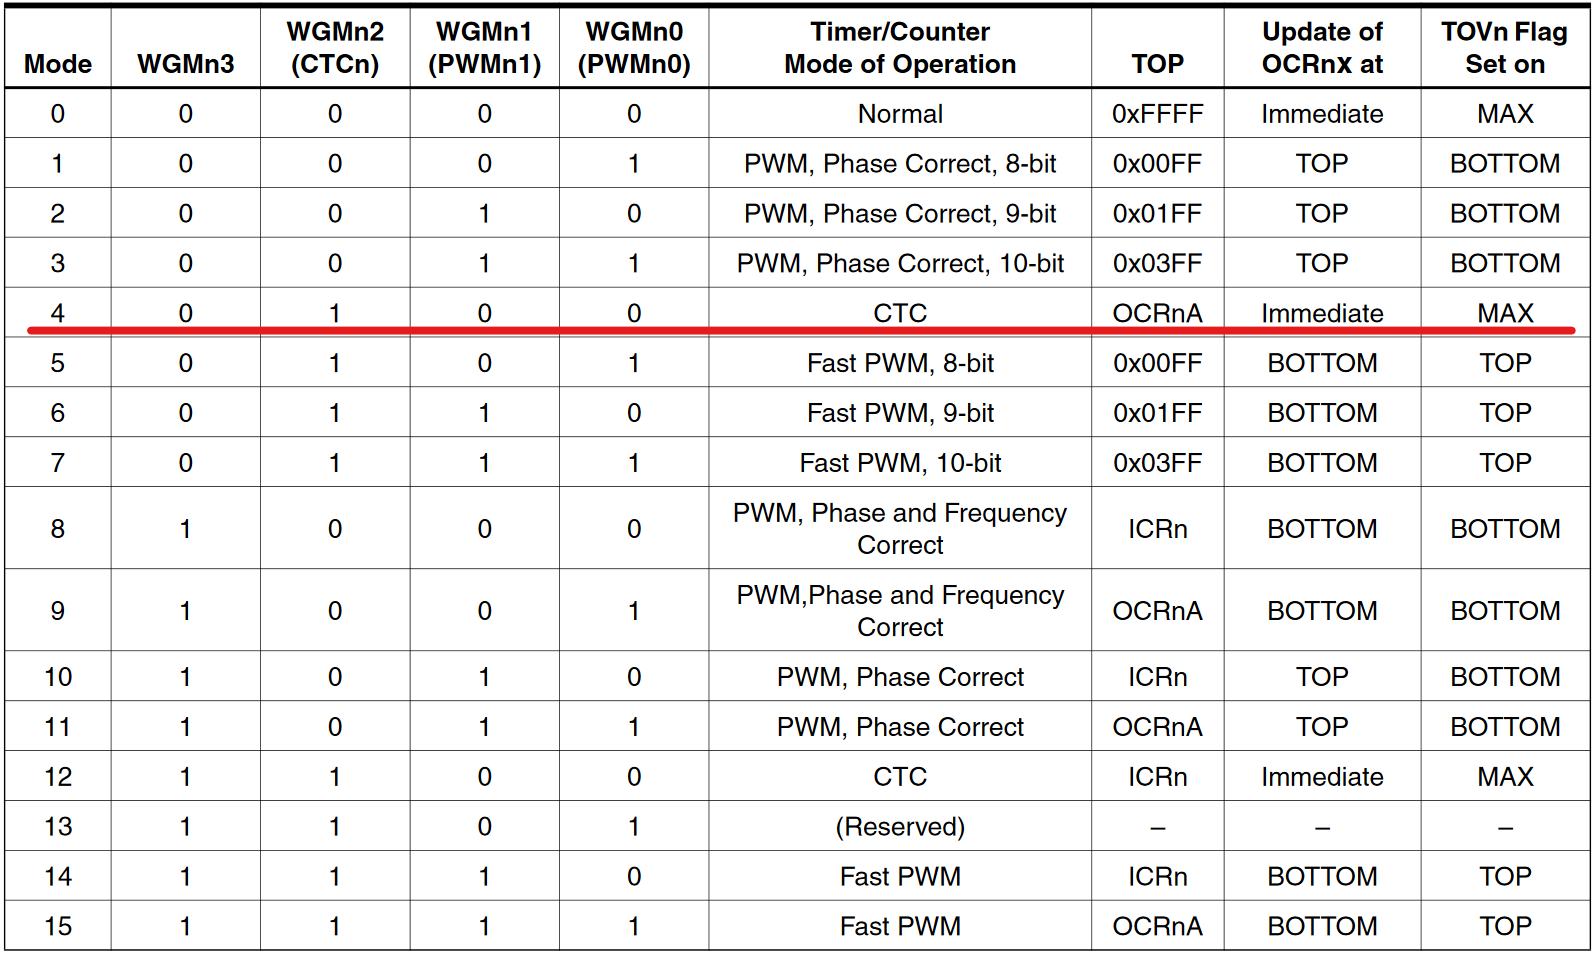
\includegraphics[width=\textwidth]{graphics/Timer_CTC_Mode}
	\caption{Timing-Diagramm CTC-Mode. OCnx nicht angeschlossen, Pin wird softwaremässig getoggelt.\cite[S.145]{atmel_atmel_2014}}
	\label{fig:Timer_CTC_Mode}
\end{figure}

\begin{figure}[h!]
	\centering
	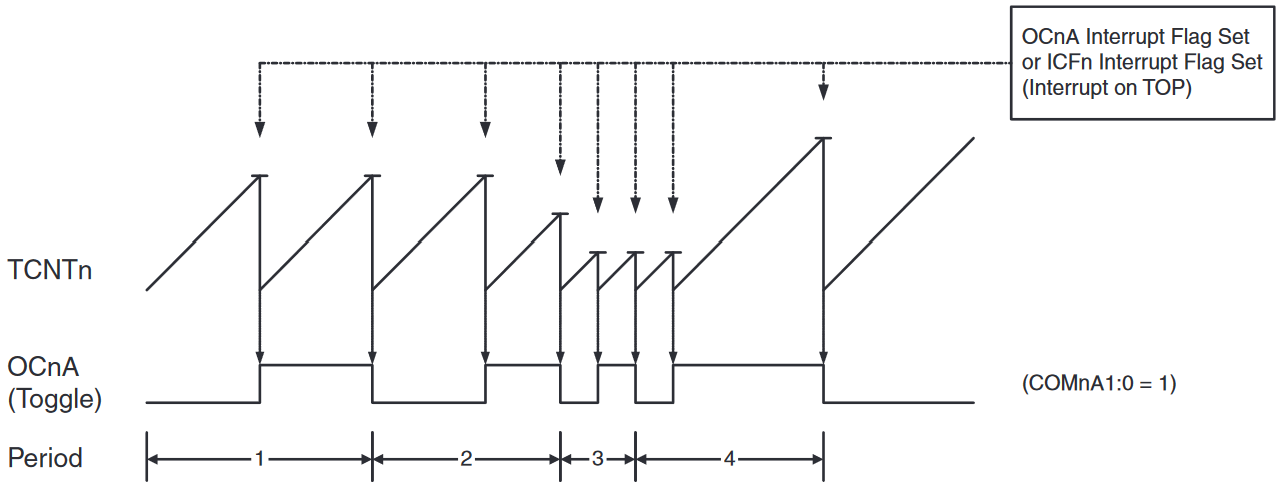
\includegraphics[width=\textwidth]{graphics/Timer_CTC_Timing_Diagram}
	\caption{Timing-Diagramm CTC-Mode. OCnx nicht angeschlossen, Pin wird softwaremässig getoggelt.\cite[S.146]{atmel_atmel_2014}}
	\label{fig:Timer_CTC_Timing_Diagram}
\end{figure}

Der Duty-Cycle wird Prozentual zum OCRnA-Register gesetzt. Wird für den berechneten Wert ein Duty-Cycle von 50\% vorgegeben, ergibt sich für das OCRnB-Register den Wert $(1600 / 2) -1 \approx 799$. So wird nach der Hälfte der Hochzählzeit ein zweiter Compare-Interrupt ausgelöst, welcher jedoch kein Einfluss auf das Counter-Register hat. Das Verhalten ist dann wie im Fast-PWM-Mode, welcher in Abbildung \ref{fig:Timer_Fast_PWM_Timing_Diagram} zu sehen ist. Nur dass anstelle von toggeln des OCnx-Pins softwaremässig ein Pin getoggelt wird. Die Inbetriebnahme hat gezeigt, dass ein Duty-Cycle von 95\% nicht überschritten werden sollte.

\begin{figure}[h!]
	\centering
	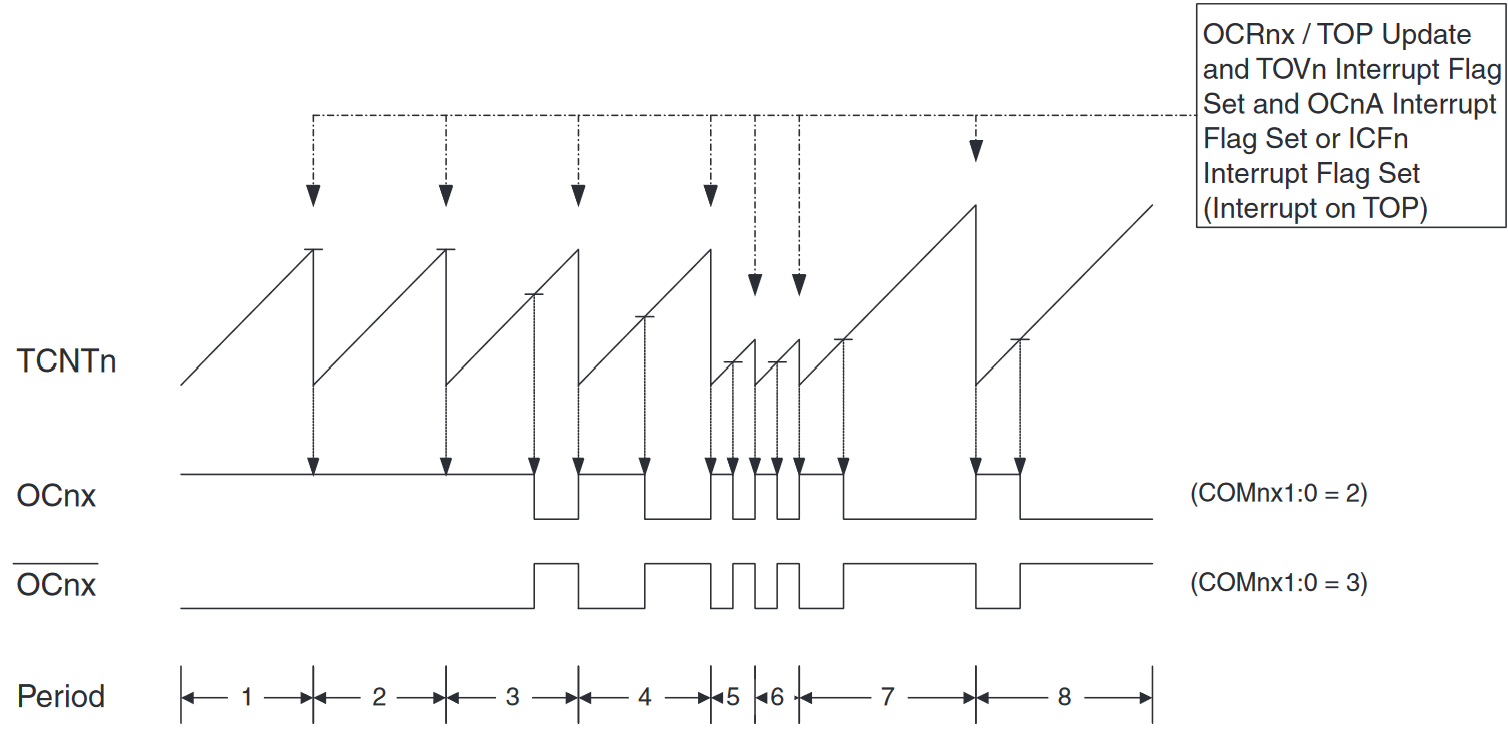
\includegraphics[width=\textwidth]{graphics/Timer_Fast_PWM_Timing_Diagram}
	\caption{Timing-Diagramm Fast-PWM-Mode. OCnx nicht angeschlossen, Pin wird softwaremässig getoggelt.\cite[S.147]{atmel_atmel_2014}}
	\label{fig:Timer_Fast_PWM_Timing_Diagram}
\end{figure}

Nun muss in beiden der erwähnten Interrupt-Routinen das gewünschte LED getoggelt werden. In der ersten Interruptroutine mit dem OCRnA-Compare-Register wird die LED eingeschaltet, in der zweiten Interruptroutine mit dem OCRnB-Compare-Register wird die LED ausgeschaltet.

Möchte man nun die Helligkeit angepasst werden, kann ein Wert zwischen 0 und OCRnA ausgewählt werden und damit das Register OCRnB beschrieben werden.

\subsubsection{Rainbow-Funktion}

Die Farbe der RGB-LED soll nun jeweils fünf Sekunden brauchen, um einen Farbteil komplett ein- oder auszuschalten, was einen sanften Übergang im Farbkreis ermöglicht.

Inspiration für den Rainbow-Algorithmus war ein Blog von Łukasz Podkalicki. \cite{podkalicki_attiny13_2016}

Im Rainbow-Loop gibt es sechs States. Zubeginn muss die grüne LED schon voll leuchten.
\begin{enumerate}
\item Start ==> Grün
\item Hochzählen des Rot-Anteils ==> Yellow
\item Runterzählen des Grün-Anteils ==> Rot
\item Hochzählen des Blau-Anteils ==> Magenta
\item Runterzählen des Rot-Anteils ==> Blau
\item Hochzählen des Grün-Anteils ==> Cyan
\item Runterzählen des Blau-Anteils ==> Grün
\item Repeat 2 - 7
\end{enumerate}

Es benötigt 1600 Schritte um einen Farbteil komplett ein- und auszuschalten. Pro Interrupt wird ein Schritt hochgezählt. Mit Formel \ref{equ:Milli_S} kann direkt berechnet werden, mit welchem Wert das Compare-Register beschrieben werden muss, sodass es fünf Sekunden geht, bis 1600 Schritte hochgezählt wurden.

\begin{equation}
OCR_{nx} = \frac{f_{clk_{I/O}}}{N \cdot f_{OC_{max}}} - 1 = \frac{16MHz}{1024 \cdot \frac{1600 Schritte}{5s}} - 1 \approx 48
\label{equ:Milli_S}
\end{equation}

Die Iteration durch den Rainbow-Modus wird folglich mit einer Frequenz von 160Hz initialisiert. In der Routine wird demnach alle 6.25ms der Duty-Cytle einer Farbe hoch oder runtergezählt, und das Timer-Compare-Register des entsprechenden LED-Timers angepasst.